\chapter{Analýza výsledků optimalizace}
\label{chap:analysis}

V této kapitole popisujeme a porovnáváme výsledky optimalizací s pomocí
optimalizačních algoritmů, které popisuje \cref{chap:optim}. 

Pro analýzu výsledků optimalizace, která vhodně popisuje kvalitu řešení je
vhodné zvolit parametry simulátoru tak, aby co nejrealističtěji popisovaly 
simulované prostředí. Tato volba je bohužel v mnoha případech značně komplikovaná,
neboť řada parametrů je definována pro snadnou práci se simulátorem a jejich 
hodnota není jednoduše dohledatelná z reálných zdrojů. Z tohoto důvodu
řadu parametrů nastavujeme empiricky, nebo pomocí porovnání výsledků simulace.


\section{Poznámka ke značení}
S ohledem na množství parametrů simulátoru a na přehlednost textu, budeme 
popisovat parametry zvolené pro analýzu ve formátu podobném
\texttt{JSON}\footnote{\url{https://www.json.org/json-en.html}}, vždy s
klíčem udávajícím jméno parametru v našem simulátoru a polem zkoumaných hodnot.
\Cref{subsec:parametry_programu} obsahuje popis všech parametrů v
simulátoru.
Tedy například jako:

\begin{verbatim}
    "carConsumption" : [0.001],
    "carVelocity" : [1, 2],
    "numStations" : [300]
\end{verbatim}

V příkladu je specifikováno, že analyzujeme všechny kombinace hodnot parametrů
simulátoru takové, že počet nabíjecích stanic je vždy $300$, průměrná spotřeba 
je vždy $0.001$ a průměrná rychlost všech vozidel je buď $1$ nebo $2$. Celkem
tedy v tomto příkladě analyzujeme 2 různé varianty nastavení simulátoru.


\section{Výběr parametrů simulátoru}
\label{sec:vyber_parametru}

Simulátor navržen v naší práci nabízí širokou škálu nastavitelných parametrů.
Z tohoto důvodu před analýzou jednotlivých optimalizačních metod nejprve 
analyzujeme nastavení parametrů simulátoru a u části z nich také analyzujeme 
správnost implementace simulátoru s ohledem na zvolený parametr.
Vzhledem k výpočetní náročnosti simulace dopravy je pro nás prakticky nemožné
podrobně analyzovat všechny parametry. Analyzujeme proto jen část námi vybraných 
parametrů.

\subsection{Popis analýzy}

Pro zvolené kombinace parametrů vždy simulujeme 10 náhodných modelů splňujících
požadované parametry. Jejich výsledky následně průměrujeme a analyzujeme.

Pouze na našem rozhodnutí bez jakékoli analýzy jsme pevně zvolili následující
parametry:

\begin{Verbatim}
    "simulationTime" : [1000],
    "segmentLength" : [1],
    "stationCapacity" : [1],
    "batteryTresholdLambda" : [20],
    "carBatteryMean" : [0.7],
    "carBatteryDeviation" : [0.2],
    "carStartBatteryBottomLimit" : [0.5],
    "notChargingTreshold" : [0.7],
    "chargingWaitingTime" : [5],
    "meanChargingLevel" : [0.5]
\end{Verbatim}

Většina těchto parametrů ovlivňuje simulaci pouze minimálně, pokud jsou zvoleny v rozumném
rozmezí hodnot. Za povšimnutí stojí nahlédnout na parametr \texttt{segmentLength},
značící délku hran v grafu v kilometrech a určuje přesnost, s jakou jsme schopni
v simulované dopravní síti pracovat (v našem případě je to 1 kilometr). Dále je vhodné
zmínit, že volíme pevnou dobu úplného nabití vozidla na 5 minut, která
je optimistickým předpokladem s ohledem na reálné 
hodnoty\footnote{\url{https://pod-point.com/guides/driver/how-long-to-charge-an-electric-car}}
a každá nabíjecí stanice má pouze 1 nabíjecí slot. Tyto hodnoty volíme,
protože s pomocí našich optimalizačních algoritmů neumíme efektivně optimalizovat čas 
čekání na stanici a nemusíme se jimi výrazně zabývat.

Asi nejdůležitějším zvoleným pevným parametrem je doba simulace. Tu nastavujeme na
1000 minut, tedy 16 hodin a 40 minut. Pro tuto hodnotu se rozhodujeme, neboť se jedná
o dostatečně dlouhý časový úsek a zároveň je simulace upočítatelná v rozumném čase.

Parametry simulátoru, u nichž zkoumáme více variant jsou:

\begin{Verbatim}
    "numStations" : [300],
    "numClosestStations" : [1, 3, 5, 10], 
    "carConsumption" : [0.0001, 0.001],
    "exponentialLambdaCities" : [0.001, 0.01, 0.1],
    "exponentialLambdaDepartures" : [1000, 10000],
    "endCityRatio" : [0.01, 0.1, 1, 10, 100],
    "chargingTreshold" : [0.3, 0.5, 0.7],
    "batteryTolerance" : [0.0, 0.05, 0.1],
    "carVelocity" : [1, 1.5, 2, 3, 5]
\end{Verbatim}

Mezi parametry výše zařazujeme také celkový počet nabíjecích stanic, který nastavujeme
na hodnotu 300. Důvodem této volby je potřeba co nejefektivnější simulace, protože 
počet zkoumaných kombinací parametrů je velmi vysoký. Počet nabíjecích stanic podrobněji
analyzujeme až v analýze optimalizačních algoritmů.

Ze zkoumaných parametrů nás zajímá především vliv parametru udávající počet nabíjecích
stanic pro výběr vhodné nabíjecí stanice vozidlem 
(viz. \cref{subsec:zajizdeni_na_nabijecku}).
Zajímá nás především do jakých hodnot má rostoucí počet vybíraných nabíjecích stanic
zásadní vliv na počtu vozidel, kterým se vybila baterie. 

Výsledky experimentů bohužel nejsou moc vypovídající a paradoxně vycházely nejhůře
výsledky pro hodnotu 10 parametru \texttt{numClosestStations}.
To si odůvodňujeme volbou pouze 300 nabíjecích stanic v modelu
s celkový počet měst 521. Vzhledem ke strategii zajíždění vozidel na 
nabíječku, jež významně závisí na počtu měst, lze význam parametru pozorovat spíše až u 
rostoucího počtu nabíjecích stanic překračujícího počet měst na mapě. Při dalších experimentech, v
nichž jsme pracovali s vyšším počtem nabíjecích stanic jsme již pozorovali výraznější zlepšení
kvality řešení s rostoucím počtem stanic pro výběr. Z těchto experimentů bohužel
nemáme dostatek dat pro ilustraci.

Pro ilustraci přikládáme dvě tabulky popisující závislost počtu vybitých vozidel v simulaci, z nichž 
vozidlo vybírá (viz. \cref{tab:vyber_stanic_vybita_vozidla}), a na 
průměrné době cestování (viz. \cref{tab:vyber_stanic_doba_cestovani}). Tabulky
pracují s výsledky simulací, v nichž jsme volili pouze parametry s následujícími hodnotami:

\begin{Verbatim}
    "numStations" : [300],
    "numClosestStations" : [1, 5, 10], 
    "carConsumption" : [0.001],
    "exponentialLambdaCities" : [0.001, 0.01, 0.1],
    "exponentialLambdaDepartures" : [1000],
    "endCityRatio" : [0.01, 1, 100],
    "chargingTreshold" : [0.5],
    "batteryTolerance" : [0.05],
    "carVelocity" : [1.5]
\end{Verbatim}

\begin{table}
% uncomment the following line if you use the fitted top captions for tables
% (see the \floatsetup[table] comments in `macros.tex`.
%\floatbox{table}[\FBwidth]{
\centering\footnotesize\sf
\begin{tabular}{llr}
\toprule
Počet stanic pro výběr & \texttt{endCityRatio} & Počet vybitých vozidel\\
\midrule
1 & 1 & 626296 \\
1 & 0.01 & 626699 \\
5 & 0.01 & 632876 \\
5 & 1 & 638826 \\
5 & 100 & 642185 \\
10 & 0.01 & 654256 \\
1 & 100 & 655669 \\
10 & 100 & 657132 \\
10 & 1 & 661079 \\
\bottomrule
\end{tabular}
%}{  % uncomment if you use the \floatbox (as above), erase otherwise
\caption{Porovnání volby variant počtu stanic z nichž vozidlo vybírá a parametru \texttt{endCityRatio},
jenž určuje důležitost vzdálenosti při generování koncového města 
(viz. \cref{subsec:parametry_programu}).
Tabulka je setříděna podle počtu vozidel, jimž se vybila baterie během simulace. V simulaci
bylo rozmístěno celkem 300 nabíjecích stanic.}
%}  % uncomment if you use the \floatbox
\label{tab:vyber_stanic_vybita_vozidla}
\end{table}


\begin{table}
% uncomment the following line if you use the fitted top captions for tables
% (see the \floatsetup[table] comments in `macros.tex`.
%\floatbox{table}[\FBwidth]{
\centering\footnotesize\sf
\begin{tabular}{llr}
\toprule
Počet stanic pro výběr & \texttt{endCityRatio} & Průměrná doba cestování (v minutách)\\
\midrule
1 & 100 & 97.6049 \\
10 & 100 & 111.366 \\
1 & 0.01 & 114.14 \\
10 & 1 & 114.739 \\
1 & 1 & 114.947 \\
5 & 0.01 & 115.651  \\
5 & 100 & 115.877  \\
5 & 1 & 115.981 \\
10 & 0.01 & 117.251 \\
\bottomrule
\end{tabular}
%}{  % uncomment if you use the \floatbox (as above), erase otherwise
\caption{Porovnání volby variant počtu stanic z nichž vozidlo vybírá a parametru \texttt{endCityRatio},
jenž určuje důležitost vzdálenosti při generování koncového města 
(viz. \cref{subsec:parametry_programu}).
Tabulka je setříděna podle průměrné doby cestování vozidel v simulaci. V simulaci
bylo rozmístěno celkem 300 nabíjecích stanic.}
%}  % uncomment if you use the \floatbox
\label{tab:vyber_stanic_doba_cestovani}
\end{table}


Většina dalších parametrů ovlivňovala simulaci očekávaným způsobem a vzhledem k jejich vysokém
počtu je v tomto textu podrobněji neanalyzujeme. K práci jsou v příloze dodány veškeré výsledky
simulací ve formě tabulky, jež popisuje volbu parametrů a obsahuje podrobnější informace
o výsledcích simulace (viz. \cref{chap:prilohy}).


\section{Analýza optimalizačních metod}

Na základě výsledků experimentů ze \cref{sec:vyber_parametru} volíme pro další experimenty
následující parametry simulátoru:

\begin{verbatim}
    "simulationTime" : [1000],
    "segmentLength" : [1],
    "numClosestStations" : [10],
    "carConsumption" : [0.001],
    "stationCapacity" : [1],
    "exponentialLambdaCities" : [0.005],
    "exponentialLambdaDepartures" : [1000],
    "endCityRatio" : [1],
    "batteryTresholdLambda" : [20],
    "carBatteryMean" : [0.7],
    "carBatteryDeviation" : [0.2],
    "carStartBatteryBottomLimit" : [0.5],
    "chargingTreshold" : [0.5],
    "notChargingTreshold" : [0.8],
    "batteryTolerance" : [0.05],
    "carVelocity" : [1.5],
    "chargingWaitingTime" : [5],
    "meanChargingLevel" : [0.5]
\end{verbatim}

Pro správné chování optimalizačních metod potřebujeme vhodně zvolit parametry pro 
výpočet ztrátové funkce. Ty volíme tak, aby hodnota ztrátové funkce odrážela 
především počet vybitých vozidel v simulaci. Část hodnoty přidělujeme také
počtu nabíjecích stanic. Parametry dalších složek ztrátové funkce volíme tak, aby
měly na hodnotu ztrátové funkce minimální vliv. Tento postup je motivován
myšlenkami, které popisuje \cref{sec:loss}. Parametry ztrátové funkce volíme
následovně:

\begin{verbatim}
    "stationNumberParameter" : [100],
    "runDownParameter" : [100],
    "durationParameter" : [1],
    "batteryDifferenceParameter" : [1],
    "waitingTimesParameter" : [1]
\end{verbatim}

Nabízí se zde také možnost volby většího zapojení počtu nabíjecích stanic v 
hodnotě ztrátové funkce pro optimalizaci počtu stanic. Z experimentů však
pozorujeme, že tato změna nemá výraznější vliv na výsledcích optimalizace 
(pokud nevolíme výrazně vyšší hodnoty parametru \texttt{stationNumberParameter}).
Zároveň v následující analýze téměř nikdy nezmiňujeme další parametry pro
výpočet chybové funkce, protože tyto hodnoty byly často velmi podobné, nebo
z nich nebyla patrná závislost na ostatních parametrech optimalizace či simulátoru.



\subsection{Poznámka k výsledkům experimentů}
V rozboru jednotlivých optimalizačních metod často v tabulkách vypisujeme jen
vybranou podmnožinu výsledků. Postup při výběru je popsán u každé tabulky. K tomuto kroku
přistupujeme, neboť vetšina experimentů pracuje s mnoha variantami parametrů a výpis všech 
by byl zbytečně nepřehledný. Kompletní výsledky se nacházení v příloze práce 
(viz. \cref{chap:prilohy}). Výsledky některých kombinací parametrů nejsou
jsou ve výsledcích zahrnuty, protože experimenty nebylo možné dokončit z
důvodu nedostatečné výpočetní výkonnosti stroje, na němž jsme experimenty pouštěli.


\subsection{Náhodný přístup}

O optimalizačních algoritmech musíme vhodným způsobem rozhodnout, zda zlepšují
kvalitu řešení problému. K tomuto rozhodnutí potřebujeme referenční hodnotu, kterou
získáváme z dat získaných opakovanými simulacemi dopravy s náhodně rozmístěnými
stanicemi. 

Stanice generuje stejným způsobem jako počáteční pozici vozidla 
(\cref{subsec:generovani_vozidel}). Tedy nejprve vygenerujeme město, kterému bude
stanice náležet, a následně v daném městě uniformně náhodně generujeme 
vrchol grafu, jenž určuje pozici stanice.

\Cref{tab:vysledky_nahodne} znázorňuje výsledky náhodného přístupu.

\begin{table}
% uncomment the following line if you use the fitted top captions for tables
% (see the \floatsetup[table] comments in `macros.tex`.
%\floatbox{table}[\FBwidth]{
\centering\footnotesize\sf
\begin{tabular}{lr}
\toprule
Počet nabíjecích stanic & Počet vybitých vozidel\\
\midrule
4000 & 586865  \\
2000 & 590083 \\
1000 & 631222 \\
500 & 687167  \\
300 & 753241 \\
\bottomrule
\end{tabular}
%}{  % uncomment if you use the \floatbox (as above), erase otherwise
\caption{Počet vybitých vozidel v simulaci v závislosti na počtu nabíjecích stanic při náhodném
rozdělení stanic.}
%}  % uncomment if you use the \floatbox
\label{tab:vysledky_nahodne}
\end{table}


\subsection{Optimalizace hladovým algoritmem}

Při analýze hladového optimalizačního (\cref{sec:greedy}) přístupu zvažujeme
varianty parametrů:
\begin{verbatim}
    "lossDifferenceTreshold" : [100],
    "greedyMaxIterations" : [20],
    "greedyNumThrowAway" : [1, 5, 10]
\end{verbatim}

Výsledky vykazují prokazatelně menší hodnoty počtu vybitých vozidel než při
náhodném přístupu a v případě malého počtu počátečních nabíjecích stanic,
také poměrně zásadní redukci výsledného počtu stanic, při níž nedošlo k výraznému
nárustu počtu vybitých vozidel. \Cref{tab:vysledky_greedy} popisuje 
vybrané hodnoty počtu vybitých vozidel a výsledného počtu nabíjecích stanic v 
závislosti na počtu nabíjecích stanic na začátku optimalizace.

\begin{table}
% uncomment the following line if you use the fitted top captions for tables
% (see the \floatsetup[table] comments in `macros.tex`.
%\floatbox{table}[\FBwidth]{
\centering\footnotesize\sf
\begin{tabular}{lllrr}
\toprule
$s_0$ & $iter_{max}$ & $r$ & Počet stanic & Počet vybitých vozidel\\
\midrule
4000 & 20 & 5 & 4000 & 515166 \\
4000 & 20 & 1 & 4000 & 516282 \\
2000 & 20 & 2 & 2000 & 516668 \\
2000 & 20 & 1 & 2000 & 517458 \\
1000 & 20 & 2 & 1000 & 571645 \\
1000 & 20 & 5 & 1000 & 572448 \\
500 & 20 & 5 & 495 & 645667 \\
500 & 20 & 2 & 498 & 646647 \\
300 & 20 & 2 & 284 & 678159 \\
300 & 20 & 5 & 285 & 687528 \\
\bottomrule
\end{tabular}
%}{  % uncomment if you use the \floatbox (as above), erase otherwise
\caption{Počet vybitých vozidel v simulaci a výsledný počet nabíjecích stanic v závislosti na 
počátečním počtu nabíjecích stanic při optimalizaci hladovým algoritmem. V tabulce zahrnujeme
vybrané hodnoty pro různé parametry optimalizace. Mezi vybrané hodnoty patří ty v níž byl
nejnižší a nejvyšší počet vybitých vozidel a ty v níž bylo dosaženo nejnižšího výsledného počtu stanic.
Výsledky jsou seřazeny podle počtu vybitých vozidel v simulaci. Hodnoty $s_0$ značí
počáteční počet nabíjecích stanic, $iter_{max}$ maximální počet iterací algoritmu a 
$r$ maximální rozdíl v počtu stanic mezi iteracemi.}
%}  % uncomment if you use the \floatbox
\label{tab:vysledky_greedy}
\end{table}


\subsection{Optimalizace genetickým algoritmem}
Při analýze optimalizace genetickým algoritmem (\cref{sec:genetic_optim})
zvažujeme parametry:

\begin{verbatim}
    "geneticPopulationSize" : [10],
    "geneticNumGenerations" : [10, 20],
    "geneticNumBestSelection" : [0, 4],
    "geneticTournamentSelectionTreshold" : [0.7, 0.9],
    "geneticMutationTreshold" : [0.0001, 0.001, 0.01],
    "geneticMemberSizeVariance" : [10]
\end{verbatim}

Výsledky prokazují, že optimalizace výrazným způsobem snižuje počet vybitých
vozidel v simulaci. \Cref{tab:vysledky_genetic} popisuje vybrané hodnoty počtu
vybitých vozidel a výsledného počtu nabíjecích stanic v závislosti na počtu 
nabíjecích stanic na začátku optimalizace.

Je potřeba zmínit, že výsledky optimalizace by pravděpodobně mohly dosahovat
lepších výsledků pro větší počet jedinců v populaci a větší počet generací.
Vzhledem k výpočetní náročnosti, jsme bohužel experimenty na těchto parametrech 
nebyli schopni realizovat.


\begin{table}
% uncomment the following line if you use the fitted top captions for tables
% (see the \floatsetup[table] comments in `macros.tex`.
%\floatbox{table}[\FBwidth]{
\centering\footnotesize\sf
\begin{tabular}{llllllrr}
\toprule
$s_0$ & $pop_{size}$ & $num_{gen}$ & $k$ & $p_{sel}$ &$p_{mut}$ & Počet stanic & Počet vybitých vozidel\\
\midrule
2000 & 10 & 10 & 4 & 0.9 & 0.01 & 2003 & 495100 \\
4000 & 10 & 10 & 0 & 0.9 & 0.01 & 3997 & 496395 \\
4000 & 10 & 10 & 0 & 0.7 & 0.0001 & 4001 & 498511 \\
2000 & 10 & 10 & 0 & 0.9 & 0.0001 & 1987 & 500384 \\
4000 & 10 & 20 & 4 & 0.9 & 0.01 & 3997 & 506130 \\
2000 & 10 & 20 & 4 & 0.9 & 0.0001 & 2001 & 506735 \\
1000 & 10 & 10 & 4 & 0.7 & 0.01 & 1001 & 526682 \\
1000 & 10 & 10 & 4 & 0.9 & 0.0001 & 997 & 537434 \\
1000 & 10 & 10 & 0 & 0.7 & 0.0001 & 1002 & 539771 \\
500 & 10 & 10 & 0 & 0.7 & 0.01 & 501 & 594346 \\
500 & 10 & 10 & 4 & 0.9 & 0.01 & 503 & 594541 \\
500 & 10 & 10 & 0 & 0.7 & 0.0001 & 497 & 595689 \\
500 & 10 & 20 & 4 & 0.9 & 0.01 & 503 & 606166 \\
300 & 10 & 10 & 4 & 0.7 & 0.01 & 301 & 640300 \\
300 & 10 & 10 & 4 & 0.7 & 0.0001 &  300 & 643191 \\
300 & 10 & 10 & 0 & 0.7 & 0.0001 & 301 & 652122 \\
\bottomrule
\end{tabular}
%}{  % uncomment if you use the \floatbox (as above), erase otherwise
\caption{Počet vybitých vozidel v simulaci a výsledný počet nabíjecích stanic v 
závislosti na počátečním počtu nabíjecích stanic při optimalizaci genetickým algoritmem. 
V tabulce zahrnujeme vybrané hodnoty pro různé parametry optimalizace. Mezi vybrané 
hodnoty patří ty v níž byl nejnižší a nejvyšší počet vybitých vozidel a ty v níž bylo
dosaženo nejnižšího a nejvyššího výsledného počtu stanic.
Výsledky jsou seřazeny podle počtu vybitých vozidel v simulaci. Hodnoty $s_0$ značí
počáteční počet nabíjecích stanic, $pop_{size}$ velikost populace v GA, $num_{gen}$
počet generací GA, $k$ počet nejlepších výsledků pro zkopírování do nové
populace GA, $p_{sel}$ pravděpodobnost výběru lepšího jedince v turnajové selekci a
$p_{mut}$ značí pravděpodobnost mutace jedné stanice.}
%}  % uncomment if you use the \floatbox
\label{tab:vysledky_genetic}
\end{table}


\subsection{Optimalizace s pomocí k-means}

Poslední zkoumaný přístup je optimalizace pomocí algoritmu k-means 
(\cref{sec:kmeans_optim}) zvažujeme parametry:

\begin{verbatim}
    "kMeansNumIterationsOneRun" : [10, 20, 50, 100],
    "kMeansNumGenerations" : [2, 10, 20, 50]
\end{verbatim}

Výsledky tohoto optimalizačního přístupu neprokazují zlepšení. Dokonce v našich
experimentech dosahuje tento algorimus horších výsledků než náhodný přístup.
\Cref{tab:vysledky_kmeans} popisuje vybrané hodnoty počtu
vybitých vozidel v závislosti na počtu nabíjecích stanic na začátku optimalizace.
Z výsledků můžeme nahlédnout, že kvalita řešení roste s počtem iterací
algoritmu k-means i s počtem generací modelů (viz. \cref{sec:kmeans_optim}).
Je tak tedy možné, že v případě vyššího počtu opakování by optimalizace dosahovala
lepších výsledků.


\begin{table}
% uncomment the following line if you use the fitted top captions for tables
% (see the \floatsetup[table] comments in `macros.tex`.
%\floatbox{table}[\FBwidth]{
\centering\footnotesize\sf
\begin{tabular}{lllr}
\toprule
$s_0$ & $means_{iter}$ & $sim_{iter}$ & Počet vybitých vozidel\\
\midrule
4000 & 20 & 50 & 594054 \\
4000 & 10 & 10 & 595606 \\
2000 & 20 & 50 & 601595 \\
2000 & 10 & 2 & 603219 \\
1000 & 50 & 10 & 645418 \\
1000 & 20 & 2 & 647815 \\
500 & 50 & 20 & 714368 \\
500 & 50 & 2 & 716731 \\
\bottomrule
\end{tabular}
%}{  % uncomment if you use the \floatbox (as above), erase otherwise
\caption{Počet vybitých vozidel v simulaci v závislosti na počátečním počtu 
nabíjecích stanic při optimalizaci algoritmem k-means. V tabulce zahrnujeme 
vybrané hodnoty pro různé parametry optimalizace. Mezi vybrané 
hodnoty patří ty v níž byl nejnižší a nejvyšší počet vybitých vozidel.
Výsledky jsou seřazeny podle počtu vybitých vozidel v simulaci. Hodnoty $s_0$ značí
počáteční počet nabíjecích stanic, $means_{iter}$ počet iterací jednoho cyklu algoritmu
k-means a $sim_{iter}$ počet proběhlých simulací modelu (mezi spuštěním algoritmů k-means). }
%}  % uncomment if you use the \floatbox
\label{tab:vysledky_kmeans}
\end{table}


\subsection{Porovnání optimalizačních metod}

Na základě výsledků experimentů docházíme k závěru, že optimalizace za pomoci
genetického algoritmu a optimalizace hladovým přístupem dosahují lepších výsledků,
než náhodný přístup. Na druhou stranu optimalizace za pomoci algoritmu k-means
vykazuje dokonce horší výsledky než náhodný přístup. Tuto skutečnost si odůvodňujeme
velkou mírou aproximace, s níž algoritmus pracuje, a malým počtem opakování algoritmu
k-means. Dále je také potřeba zmínit, že například optimalizace pomocí genetického
algoritmu, by pravděpodobně dosahovala lepších řešení pro větší velikost populace
a počet generací. Tento případ, jsme ale s ohledem na výpočetní náročnost simulace
dopravy nebyli schopni realizovat. Dále můžeme nahlédnout, že kolem počtu 2000 stanic
se počet vybitých vozidel ustálil a není tak potřeba přidávat do mapy více stanic.

\cref{fig:porovnani_optimalizaci} znázorňujeme 
porovnání výsledků jednotlivých metod pomocí počtu použitých nabíjecích stanic a 
počtu vybitých vozů.


\begin{figure}
    \centering
    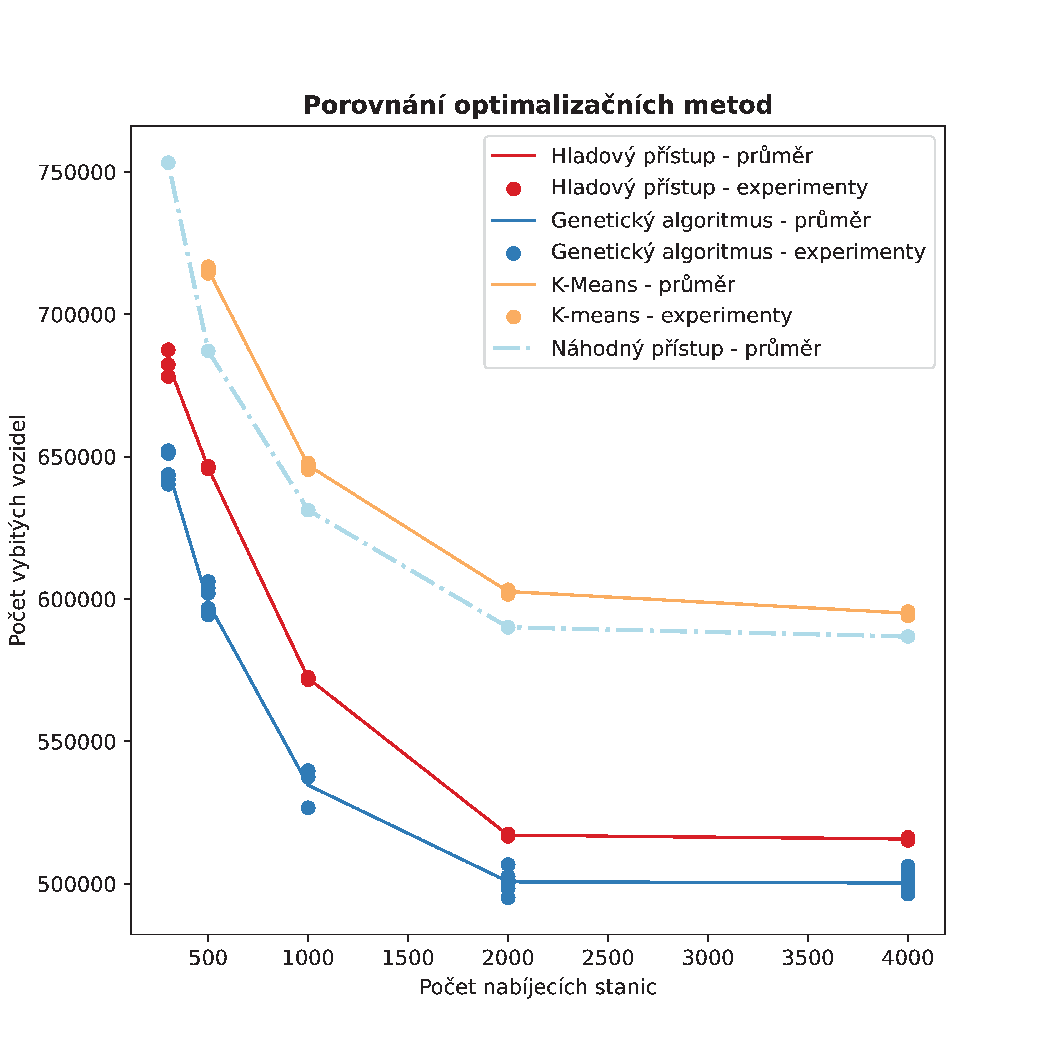
\includegraphics[width=1\linewidth]{img/pdfa-optim_compare.pdf}
    \caption{Porovnání různých optimalizačních metod. Optimalizační metody barevně
    rozlišujeme. Body v grafu znázorňují výsledky jednotlivých experimentů. Čárové
    grafy propojují průměrné hodnoty počtu vybitých vozidel při stejném počtu
    nabíjecích stanic. Čerchovaný čárový graf značí výsledky náhodného přístupu.}
    \label{fig:porovnani_optimalizaci}
\end{figure}



\section{Pomocné nástroje pro analýzu výsledků}

S ohledem na velké množství parametrů simulátoru a výpočetní náročnosti simulace
jsme se rozhodli využít služeb organizace 
Metacentrum\footnote{\url{https://metavo.metacentrum.cz/}}. Za pomoci
této organizace jsme schopni otestovat stovky variant parametrů.
Vzhledem k množštví zkoumaných variant, je ale pro praktické použití potřeba 
zautomatizovat proces nastavování zvolených parametrů a vytváření úloh pro spuštění na 
Metacentru simulací se zvolenými parametry a následnou analýzu výsledků simulací.
K tomuto účelu jsme vytvořili pomocný program v jazyce Python 
(viz. \cref{chap:prilohy}). Tento program připravuje 
potřebné skripty pro spouštění jednotlivých úloh v Metacentru a 
umožňuje jednoduché zobrazení výsledků simulace s možností zkoumání 
námi zvolených parametrů simulace a setřídění výsledků dle zvoleného parametru.
